\documentclass[journal, a4paper]{IEEEtran}

% some very useful LaTeX packages include:

%\usepackage{cite}      % Written by Donald Arseneau
                        % V1.6 and later of IEEEtran pre-defines the format
                        % of the cite.sty package \cite{} output to follow
                        % that of IEEE. Loading the cite package will
                        % result in citation numbers being automatically
                        % sorted and properly "ranged". i.e.,
                        % [1], [9], [2], [7], [5], [6]
                        % (without using cite.sty)
                        % will become:
                        % [1], [2], [5]--[7], [9] (using cite.sty)
                        % cite.sty's \cite will automatically add leading
                        % space, if needed. Use cite.sty's noadjust option
                        % (cite.sty V3.8 and later) if you want to turn this
                        % off. cite.sty is already installed on most LaTeX
                        % systems. The latest version can be obtained at:
                        % http://www.ctan.org/tex-archive/macros/latex/contrib/supported/cite/

\usepackage{graphicx}   % Written by David Carlisle and Sebastian Rahtz
                        % Required if you want graphics, photos, etc.
                        % graphicx.sty is already installed on most LaTeX
                        % systems. The latest version and documentation can
                        % be obtained at:
                        % http://www.ctan.org/tex-archive/macros/latex/required/graphics/
                        % Another good source of documentation is "Using
                        % Imported Graphics in LaTeX2e" by Keith Reckdahl
                        % which can be found as esplatex.ps and epslatex.pdf
                        % at: http://www.ctan.org/tex-archive/info/

%\usepackage{psfrag}    % Written by Craig Barratt, Michael C. Grant,
                        % and David Carlisle
                        % This package allows you to substitute LaTeX
                        % commands for text in imported EPS graphic files.
                        % In this way, LaTeX symbols can be placed into
                        % graphics that have been generated by other
                        % applications. You must use latex->dvips->ps2pdf
                        % workflow (not direct pdf output from pdflatex) if
                        % you wish to use this capability because it works
                        % via some PostScript tricks. Alternatively, the
                        % graphics could be processed as separate files via
                        % psfrag and dvips, then converted to PDF for
                        % inclusion in the main file which uses pdflatex.
                        % Docs are in "The PSfrag System" by Michael C. Grant
                        % and David Carlisle. There is also some information
                        % about using psfrag in "Using Imported Graphics in
                        % LaTeX2e" by Keith Reckdahl which documents the
                        % graphicx package (see above). The psfrag package
                        % and documentation can be obtained at:
                        % http://www.ctan.org/tex-archive/macros/latex/contrib/supported/psfrag/

%\usepackage{subfigure} % Written by Steven Douglas Cochran
                        % This package makes it easy to put subfigures
                        % in your figures. i.e., "figure 1a and 1b"
                        % Docs are in "Using Imported Graphics in LaTeX2e"
                        % by Keith Reckdahl which also documents the graphicx
                        % package (see above). subfigure.sty is already
                        % installed on most LaTeX systems. The latest version
                        % and documentation can be obtained at:
                        % http://www.ctan.org/tex-archive/macros/latex/contrib/supported/subfigure/

\usepackage{url}        % Written by Donald Arseneau
                        % Provides better support for handling and breaking
                        % URLs. url.sty is already installed on most LaTeX
                        % systems. The latest version can be obtained at:
                        % http://www.ctan.org/tex-archive/macros/latex/contrib/other/misc/
                        % Read the url.sty source comments for usage information.

%\usepackage{stfloats}  % Written by Sigitas Tolusis
                        % Gives LaTeX2e the ability to do double column
                        % floats at the bottom of the page as well as the top.
                        % (e.g., "\begin{figure*}[!b]" is not normally
                        % possible in LaTeX2e). This is an invasive package
                        % which rewrites many portions of the LaTeX2e output
                        % routines. It may not work with other packages that
                        % modify the LaTeX2e output routine and/or with other
                        % versions of LaTeX. The latest version and
                        % documentation can be obtained at:
                        % http://www.ctan.org/tex-archive/macros/latex/contrib/supported/sttools/
                        % Documentation is contained in the stfloats.sty
                        % comments as well as in the presfull.pdf file.
                        % Do not use the stfloats baselinefloat ability as
                        % IEEE does not allow \baselineskip to stretch.
                        % Authors submitting work to the IEEE should note
                        % that IEEE rarely uses double column equations and
                        % that authors should try to avoid such use.
                        % Do not be tempted to use the cuted.sty or
                        % midfloat.sty package (by the same author) as IEEE
                        % does not format its papers in such ways.

\usepackage{amsmath}    % From the American Mathematical Society
                        % A popular package that provides many helpful commands
                        % for dealing with mathematics. Note that the AMSmath
                        % package sets \interdisplaylinepenalty to 10000 thus
                        % preventing page breaks from occurring within multiline
                        % equations. Use:
%\interdisplaylinepenalty=2500
                        % after loading amsmath to restore such page breaks
                        % as IEEEtran.cls normally does. amsmath.sty is already
                        % installed on most LaTeX systems. The latest version
                        % and documentation can be obtained at:
                        % http://www.ctan.org/tex-archive/macros/latex/required/amslatex/math/



% Other popular packages for formatting tables and equations include:

%\usepackage{array}
% Frank Mittelbach's and David Carlisle's array.sty which improves the
% LaTeX2e array and tabular environments to provide better appearances and
% additional user controls. array.sty is already installed on most systems.
% The latest version and documentation can be obtained at:
% http://www.ctan.org/tex-archive/macros/latex/required/tools/

% V1.6 of IEEEtran contains the IEEEeqnarray family of commands that can
% be used to generate multiline equations as well as matrices, tables, etc.

% Also of notable interest:
% Scott Pakin's eqparbox package for creating (automatically sized) equal
% width boxes. Available:
% http://www.ctan.org/tex-archive/macros/latex/contrib/supported/eqparbox/

% *** Do not adjust lengths that control margins, column widths, etc. ***
% *** Do not use packages that alter fonts (such as pslatex).         ***
% There should be no need to do such things with IEEEtran.cls V1.6 and later.

\usepackage{amssymb}

% Your document starts here!
\begin{document}
\begin{titlepage}

\newcommand{\HRule}{\rule{\linewidth}{0.5mm}} % Defines a new command for the horizontal lines, change thickness here

\center % Center everything on the page
 %----------------------------------------------------------------------------------------
%	LOGO SECTION
%----------------------------------------------------------------------------------------

~\\[1cm]

\includegraphics{SCUT.png}\\[2cm] % Include a department/university logo - this will require the graphicx package

%----------------------------------------------------------------------------------------
%	TITLE SECTION
%----------------------------------------------------------------------------------------

\HRule \\[1cm]
{ \huge \bfseries The Experiment Report of \textit{Machine Learning} }\\[0.6cm] % Title of your document
\HRule \\[2cm]
%----------------------------------------------------------------------------------------
%	HEADING SECTIONS
%----------------------------------------------------------------------------------------


\textsc{\LARGE \textbf{School:} School of Software Engineering}\\[1cm]
\textsc{\LARGE \textbf{Subject:} Electronic and Information}\\[2cm]


%----------------------------------------------------------------------------------------
%	AUTHOR SECTION
%----------------------------------------------------------------------------------------

\begin{minipage}{0.4\textwidth}
\begin{flushleft} \large
\emph{Author:}\\
Weiwen Hu
\end{flushleft}
\end{minipage}
~
\begin{minipage}{0.4\textwidth}
\begin{flushright} \large
\emph{Supervisor:} \\
Mingkui Tan
\end{flushright}
\end{minipage}\\[2cm]
~
\begin{minipage}{0.4\textwidth}
\begin{flushleft} \large
\emph{Student ID:}\\
202021045611
\end{flushleft}
\end{minipage}
~
\begin{minipage}{0.4\textwidth}
\begin{flushright} \large
\emph{Grade:} \\
Graduate
\end{flushright}
\end{minipage}\\[2cm]

% If you don't want a supervisor, uncomment the two lines below and remove the section above
%\Large \emph{Author:}\\
%John \textsc{Smith}\\[3cm] % Your name

%----------------------------------------------------------------------------------------
%	DATE SECTION
%----------------------------------------------------------------------------------------

{\large \today}\\[2cm] % Date, change the \today to a set date if you want to be precise


%----------------------------------------------------------------------------------------

\vfill % Fill the rest of the page with whitespace

\end{titlepage}

% Define document title and author
	\title{Logistic Regression and Support Vector Machine}
	\maketitle

% Write abstract here
\begin{abstract}
This experiment is about two basic linear classification method: logistic regression and support vector machine, also the Batch Stochastic Gradient Descent method.
\end{abstract}

% Each section begins with a \section{title} command
\section{Introduction}
	% \PARstart{}{} creates a tall first letter for this first paragraph
\PARstart{W}{e} are conducting this experiment in hope of: 1. Compare and understand the difference between gradient descent and batch random stochastic gradient descent. 2. Compare and understand the differences and relationships between Logistic regression and linear classification. 3. Further understand the principles of SVM and practice on larger data. We are expecting to get a classification model for each of these two methods.

% Main Part
\section{Methods and Theory}
\subsection{Logistic Regression}
In statistics, the logistic model is a widely used statistical model that, in its basic form, uses a logistic function to model a binary dependent variable.

The logistic function calculates a probability. It is defined as follows:

\begin{equation}
    g(z)=\frac{1}{1+e^(-z)}.
\end{equation}

For example, given a sample with features $\mathbf{x} \in \mathbb{R}^N$, the probability that it is a positive sample can be calculated as:

\begin{equation}
    P(y=1|\mathbf{x}) = g(\mathbf{w}^\mathsf{T}\mathbf{x}).
\end{equation}

Then we can maximize the possibility of correct prediction.

\begin{equation}
    \begin{aligned}
\max \prod_{i=1}^{n} P\left(y_i | \mathbf{x}_i\right) & \Leftrightarrow \max \log \left(\prod_{i=1}^{n} P\left(y_{i} | \mathbf{x}_{i}\right)\right) \\
& \equiv \max \sum_{i=1}^{n} \log P\left(y_i | \mathbf{x}_{i}\right) \\
& \Leftrightarrow \min -\frac{1}{n} \sum_{i=1}^{n} \log P\left(y_i | \mathbf{x}_{i}\right) \\
& \equiv \min \frac{1}{n} \sum_{i=1}^{n} \log \frac{1}{P\left(y_i | \mathbf{x}_{i}\right)} \\
& \equiv \min \frac{1}{n} \sum_{i=1}^{n} \log \frac{1}{g\left(y_i \cdot \mathbf{w}^{\top} \mathbf{x}_{i}\right)} \\
& \equiv \min \frac{1}{n} \sum_{i=1}^{n} \log \left(1+e^{-y_i \cdot \mathbf{w}^{\top} \mathbf{x}_{i}}\right) \\
& \equiv \min E_{in}(\mathbf{w})
    \end{aligned}
\end{equation}

In this way, we derived the logistic loss function $E_{in}(\mathbf{w})$. We can use gradient descent method to minimize it. The gradient is:

\begin{equation}
\frac{\partial E_{in}(\mathbf{w})}{\partial \mathbf{w}}
=-\frac{1}{n} \sum_{i=1}^{n} \frac{y_i \mathbf{x}_i}{1+e^{y_i \cdot \mathbf{w}^\mathsf{T} \mathbf{x}_i}}
\end{equation}

\subsection{Support Vector Machine}

An SVM model is a representation of the examples as points in space, mapped so that the examples of the separate categories are divided by a clear gap that is as wide as possible, which is formulated by:
\begin{equation}
    \begin{array}{l}
    \max_{\mathbf{w}, b} \frac{2}{\|\mathbf{w}\|} \\
    \text {s.t.} \quad \mathbf{w}^\mathsf{T} \mathbf{x}_i+b\left\{
        \begin{array}{ll}
            \geqslant 1 & y_i=+1 \\
            \leqslant-1 & y_i=-1
        \end{array}\right.
    \end{array}
\end{equation}

But since noise and outliner is unavoidable, we must tolerant some classification mistake, so we use the hinge loss function:
\begin{equation}
    \min_{\mathbf{w}, b} \frac{\|\mathbf{w}\|^{2}}{2}+\frac{C}{n} \sum_{i=1}^{n} \max \left(0,1-y_{i}\left(\mathbf{w}^\mathsf{T} \mathbf{x}_{i}+b\right)\right),
\end{equation}
where $C$ is a hyper-parameter to balance the margin and the tolerance to outliner.

Like before, we use gradient descent to minimize this loss. The gradient is calculated to the follow:

\begin{equation}
    g_{\mathbf{w}}\left(\mathbf{x}_{i}\right)=
    \left\{\begin{array}{ll}
        -y_i \mathbf{x}_{i} & 1-y_i\left(\mathbf{w}^{\top} \mathbf{x}_{i}+b\right)>=0 \\
        0 & 1-y_i\left(\mathbf{w}^{\top} \mathbf{x}_{i}+b\right)<0
    \end{array}\right.
\end{equation}
\begin{equation}
    \frac{\partial f(\mathbf{w}, b)}{\partial\mathbf{w}}=\mathbf{w}+\frac{C}{n} \sum_{i=1}^{n} g_{\mathbf{w}}\left(\mathbf{x}_{i}\right)
\end{equation}

\section{Experiments}
\subsection{Dataset}

We use \emph{a9a} of \emph{LIBSVM} Data, including 32561 trainning and 16281 testing samples, each sample has 123 features.

\subsection{Implementation}

I use NumPy to implement all the formulas above.

I initialized parameter $\mathbf{w}$ to all zero. Parameter $C$ in SVM is set to 100. I add an extra all 1 feature to every sample, so that I don’t need to worry about the bias parameter $b$. Other hyper-parameters are listed in table~\ref{table:hyper-param}

\begin{table}[htb]
    \centering
    \caption{Hyper Parameters}
    \label{table:hyper-param}
    \begin{tabular}{l|rr}
        \hline
            & Logistic regression & SVM \\
        \hline
        Learning rate & 0.3 & 0.001 \\
        Epoch         & 30  & 20    \\
        Batch size    & 512 & 512   \\
        \hline
    \end{tabular}
\end{table}

\subsection{Results}

The experiment result is summarizes in table~\ref{table:results}

\begin{table}
    \centering
    \caption{Results}
    \label{table:results}
    \begin{tabular}{l|rr}
        \hline
            & Logistic regression & SVM \\
        \hline
        Train loss    & 0.3275 & 38.05 \\
        Test loss     & 0.3246 & 37.73 \\
        Accuracy (\%) & 85.20  & 84.64 \\
    \end{tabular}
\end{table}

Figure~\ref{figure:lr-loss}, figure~\ref{figure:lr-acc}, figure~\ref{figure:svm-loss}, figure~\ref{figure:svm-acc} show the loss fuction value and classification accuracy changing with training epoch number, respectively. The results of logistic regression and SVM are similar, both achieved arround 85\% test classification accuracy, logistic regression does slightly better.

Despite no explict regularization term added, there are no sign of over fitting. Instead, the test accuracy is even slightly higher than train accuracy. This may be caused by more noise in training set.

When tuning the parameter $C$ in SVM, I found the higher the $C$, the better the result. The large $C$ also resulted in large absolute value of the loss. This could be because these examples are not quite linearly separable, and the "clear gap" motivation of SVM does not make many sense in this scenario.

\begin{figure}
    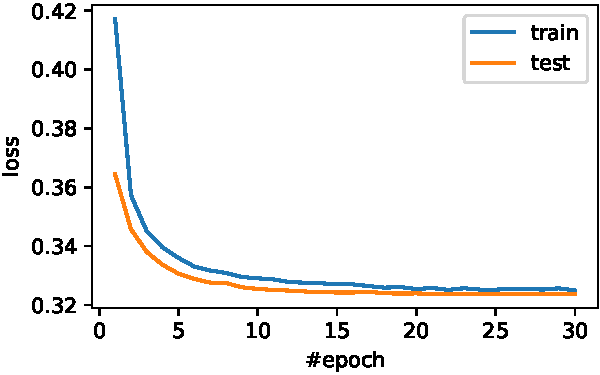
\includegraphics[width=\linewidth]{figures/lr/loss.pdf}
    \caption{Logistic Regression Loss}
    \label{figure:lr-loss}
\end{figure}

\begin{figure}
    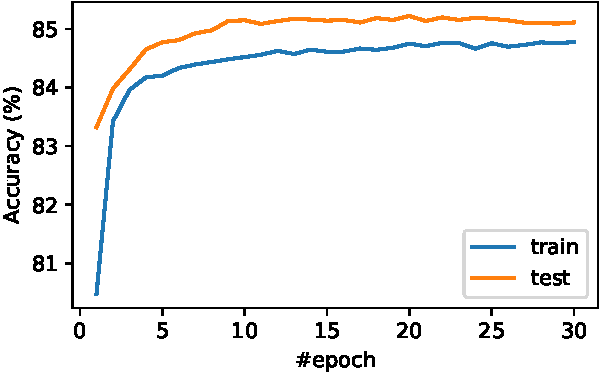
\includegraphics[width=\linewidth]{figures/lr/acc.pdf}
    \caption{Logistic Regression Accuracy}
    \label{figure:lr-acc}
\end{figure}

\begin{figure}
    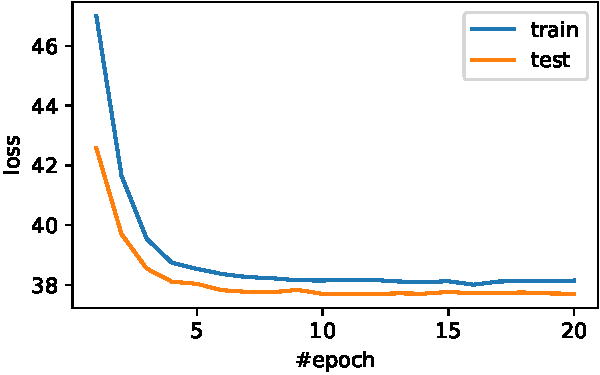
\includegraphics[width=\linewidth]{figures/svm/loss.pdf}
    \caption{SVM Loss}
    \label{figure:svm-loss}
\end{figure}

\begin{figure}
    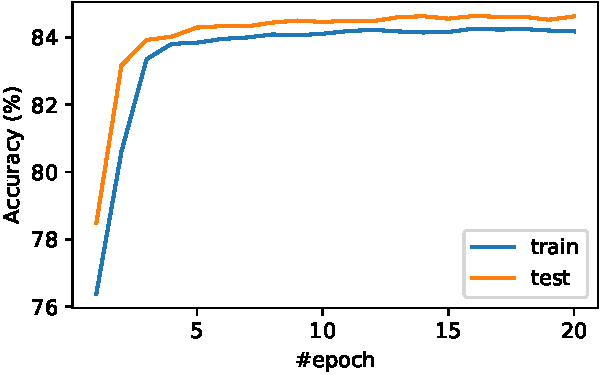
\includegraphics[width=\linewidth]{figures/svm/acc.pdf}
    \caption{SVM Accuracy}
    \label{figure:svm-acc}
\end{figure}

\section{Conclusion}

This experiment is giving expected results. I have learned the basic procedure of machine learning project and the powerful gradient descent method, as well as the logistic regression and SVM classification methods. I also get a sense of how they works compared with each other.

\end{document}
